\subsection{自同构}\label{symmeq}

我们回到第 \ref{corresp} 节的主题。$\I$ 是 $Y$ 的 $A$-模型中与拉格朗日对应 $L\subset Y\times Y'$ 相伴的界面，我们希望用 $\I$ 来定义作用在 $\H=\Hom(\B,\B_\cc)$ 上的算符。为此，我们需要“端点”，使 $\I$ 能在两个膜 $\B_\cc$ 与 $\B$ 上结束。本节聚焦于 $\B_\cc$ 及其与形变量子化的关系。量子化将在第 \ref{qtz} 节讨论。

\begin{figure}[htbp]
 \centering
 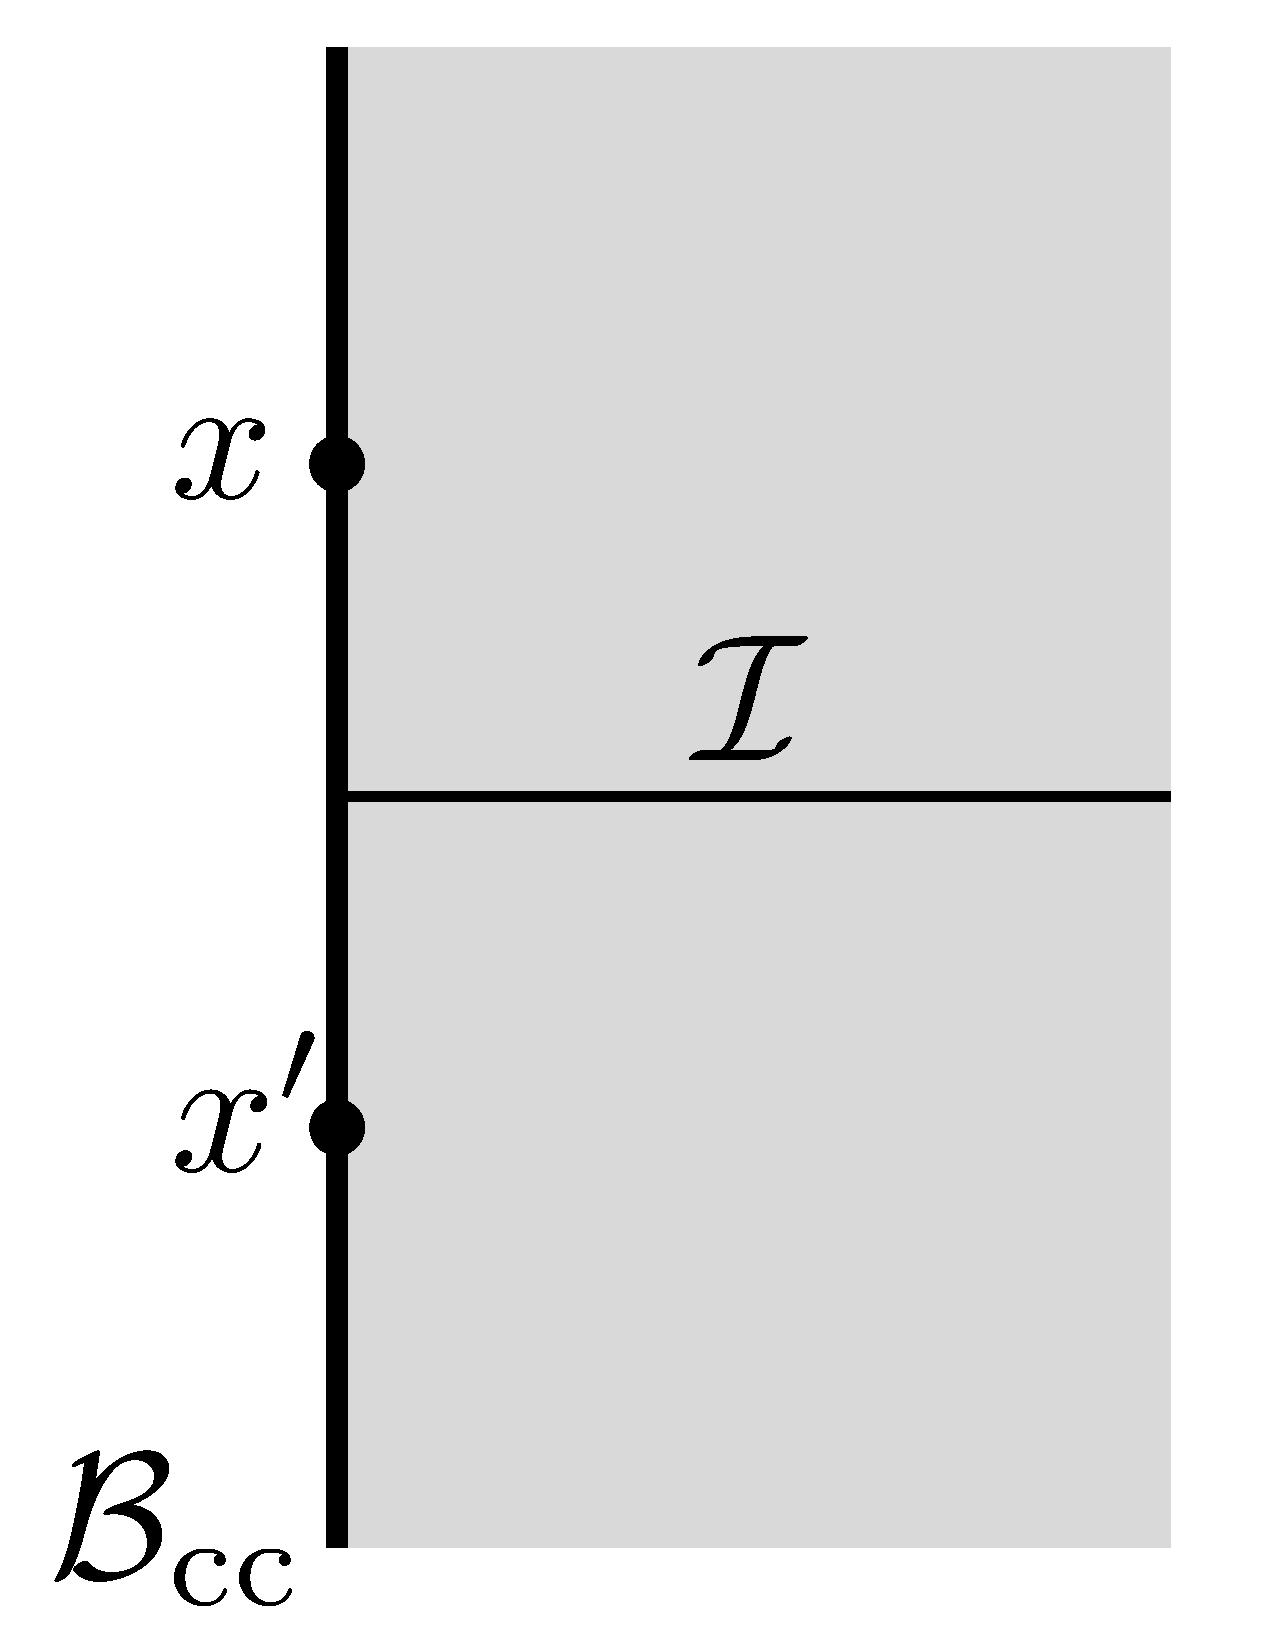
\includegraphics[width=0.28\textwidth]{figures/Pictorial.pdf}
 \caption{在界面 $\I$ 于膜 $\B_\cc$ 上的端点上方或下方插入的算符，分别给出边界算符代数 $\A$ 在 $\I$ 与 $\B_\cc$ 之间端点空间上的左作用或右作用。}\label{Pictorial}
\end{figure}

$\I$ 在 $\B_\cc$ 上结束的端点，在折叠图像中解释为 $\Hom(\h\B_\cc,\B_L)$ 的元素，其中 $\B_L$ 是支撑在 $L$ 上的拉格朗日膜，$\h\B_\cc$ 是 $Y\times Y'$ 两个因子上的余各向同性膜之积。$\Hom(\h\B_\cc,\h\B_\cc)$ 是两个 $\A=\Hom(\B_\cc,\B_\cc)$ 拷贝之积，每个因子对应一个。这两个拷贝作用在角空间 $\Hom(\h\B_\cc,\B_L)$ 上。因此展开后，两个 $\A$ 拷贝作用在 $\I$ 与 $\B_\cc$ 之间端点空间上。这一陈述有简单的图示解释（图 \ref{Pictorial}）：元素 $x\in\A$ 可以插在二维流形边界上给定端点的“下方”或“上方”。界面下方的插入对应于 $\A$ 在界面空间上的右作用，界面上方的插入对应于 $\A$ 的左作用。我们把带端点 $\alpha$ 的界面 $\I$ 记为 $\I(\alpha)$。对 $x\in\A$ 在 $\I(\alpha)$ 上的左作用或右作用，我们写 $\I(\alpha)\to x\I(\alpha)$ 或 $\I(\alpha)\to\I(\alpha)x'$。但由于 $x$ 只作用在 $\alpha$ 上，也可以更简单地写 $\alpha\to x\alpha$ 或 $\alpha\to\alpha x'$。

两个 $\A$ 拷贝在角空间 $\Hom(\h\B_\cc,\B_L)$ 上的作用，可更显式地看出如下。由附录 \ref{details}，$\Hom(\h\B_\cc,\B_L)$ 的首阶近似是
$H^0(L,\L\otimes K_L^{1/2})$，其中 $\L$ 是 $\B_L$ 的 $\CP$ 丛；为简单起见假设高阶上同调消失。由于 $L$ 嵌入 $Y\times Y'$，可以把 $H^0(L,\L\otimes K_L^{1/2})$ 的元素乘以 $Y$ 上的函数或 $Y'$ 上的函数。量子形变后，这给出两个 $\A$ 拷贝的作用。（“折叠”把代数映到反代数，其中算符按相反次序相乘；这就是为什么一个 $\A$ 拷贝以左作用、一个以右作用。）

作为一个重要的特殊情形，我们可以考虑生成代数 $\A$ 的自同构的界面 $\I$。这意味着存在角 $\alpha\in\Hom(\h\B_\cc,\B_L)$，使每个角都可唯一地写成 $x\alpha$（$x\in\A$），也可唯一地写成 $\alpha x'$（$x'\in\A$）。这一条件确定一个从 $\A$ 到自身的可逆映射 $\h\varphi$：对 $x\in\A$，$\h\varphi(x)$ 是使
$x\alpha=\alpha\h\varphi(x)$ 的 $\A$ 中元素。此外 $\h\varphi$ 可逆：对 $x\in\A$，$\h\varphi^{-1}(x)$ 是使 $\h\varphi^{-1}(x)\alpha=\alpha x$ 的 $\A$ 中元素。最后，$\h\varphi$ 是 $\A$ 的自同构，因为对 $x_1,x_2\in\A$，$x_1x_2\alpha=\alpha\h\varphi(x_1x_2)$，但另一方面 $x_1x_2\alpha=x_1\alpha\h\varphi(x_2)=\alpha\h\varphi(x_1)\h\varphi(x_2)$，故
$\h\varphi(x_1x_2)=\h\varphi(x_1)\h\varphi(x_2)$。

复常数在 $\A$ 的中心，也与界面交换，因此特别地，若 $\lambda$ 是非零复常数，则 $\lambda\alpha$ 生成与 $\alpha$ 相同的自同构。更一般地，设 $x_0$ 是 $\A$ 的任意可逆元。则对 $x\in\A$，有 $x(x_0\alpha)=x_0(x_0^{-1}xx_0)\alpha=x_0\alpha\h\varphi(x_0^{-1}xx_0)$，表明 $x_0\alpha$ 生成自同构 $x\to\h\varphi(x_0^{-1}xx_0)$。反之，若 $x_0\alpha$ 生成自同构，则角 $\alpha$ 等于某个 $x\in\A$ 的 $xx_0\alpha$，这意味着 $x_0$ 有逆 $x$。因此，若存在任何角 $\alpha$ 使给定界面生成自同构，则导致自同构的角恰为形如 $x_0\alpha$ 的角，其中 $x_0\in\A$ 可逆。

于是，在研究界面相伴的自同构时，若 $Y$ 使得常数是 $Y$ 上唯一的可逆（多项式）全纯函数，就会有一些简化。若假设 $b_1(Y)=0$，这其实是自动的；下文几处都会方便地作此假设。\footnote{设 $Y$ 上的全纯函数 $f$ 可逆，即处处不为零。则闭一形式 $\lambda=\d\log f$ 整体定义。若 $\lambda$ 恰当，$\lambda=\d u$（$u$ 为整体定义的全纯函数），则 $f=Ce^u$（$C$ 为非零常数），$f$ 在无穷远指数增长。若 $\lambda$ 不恰当，则 $\lambda$ 定义 $H^1(Y,\C)$ 的非零元素，$b_1(Y)>0$。}满足我们假设的典型例子是 $Y=\C^{2n}$，稍后我们会更仔细地研究。

现在设 $\varphi$ 是 $Y$ 的全纯辛同胚。它与复拉格朗日对应 $L\subset Y\times Y'$ 相伴，该对应参数化形如 $(y,\varphi(y))$ 的点。$L$ 有两个到 $Y$ 的映射，分别忘记 $Y\times Y'$ 的第一个或第二个因子，且每个映射都是同构。故作为复流形，$L$ 同构于 $Y$。特别地，$L$ 是复辛流形，故有典则 spin 结构。这给出折叠理论中膜 $\B_L$ 的典则选择，其 $\CP$ 丛 $\L$ 平凡；展开后它给出典则界面 $\I_L$。下文我们总作这一典则选择。又因 $b_1(Y)=0$ 且 $L$ 同构于 $Y$，$L$ 满足 $b_1(L)=0$。

反之，设 $\varphi,\varphi'$ 是 $Y$ 的两个全纯辛同胚，分别与复拉格朗日对应 $L,L'$ 及拓扑界面 $\I_\varphi,\I_{\varphi'}$ 相伴。由于 $L,L'$ 是复拉格朗日子流形，界面 $\I_\varphi$ 与 $\I_{\varphi'}$ 是 $(B,A,A)$ 型。如第 \ref{composing} 节所解释，这意味着（因 $b_1(L)=b_1(L')=0$）这些界面可以经典地合成，把它们视为 $B$-模型界面。该经典合成很容易描述。越过 $\I_\varphi$ 时，一般的 $\sigma$-模型场从 $X$ 跳到 $\varphi^*(X)$；越过 $\I_{\varphi'}$ 时，也有类似的从 $X$ 到 $\varphi'^*(X)$ 的跳变。由于我们取 $\CP$ 丛平凡，这就是全部。先越过 $\I_\varphi$ 再越过 $\I_{\varphi'}$，$X$ 先跳到 $\varphi^*(X)$，再跳到 $\varphi'^*(\varphi^*(X))$。最终结果是 $X$ 被映到 $(\varphi'\circ\varphi)^*(X)$。换言之，合成 $\I_\varphi\cdot\I_{\varphi'}$ 就是 $\I_{\varphi'\circ\varphi}$，其中 $\varphi'\circ\varphi$ 是两个辛同胚的合成。

虽然 $(B,A,A)$ 型界面可以在体内这样简单地合成，一般却没有同样简单的办法来合成它们与 $\B_\cc$ 的端点。一个例外是与 $\A$ 的自同构相关的情形。设 $\I_\varphi$ 与 $\I_{\varphi'}$ 分别带端点 $\alpha$ 与 $\alpha'$，生成 $\A$ 的自同构 $\h\varphi$ 与 $\h\varphi'$。这意味着对 $x\in\A$，有 $x\I_\varphi(\alpha)=\I_\varphi(\alpha)\h\varphi(x)$ 与 $x\I_{\varphi'}(\alpha')=\I_{\varphi'}(\alpha')\h\varphi'(x)$。合并这些关系，我们看到
\be\label{toolong}x\I_\varphi(\alpha)\I_{\varphi'}(\alpha')=\I_\varphi(\alpha)\h\varphi(x)\I_{\varphi'}(\alpha')=\I_\varphi(\alpha)\I_{\varphi'}(\alpha')\h\varphi'(\h\varphi(x)).\ee
换言之，令 $\varphi''=\varphi'\circ\varphi$，当我们合成 $\I_\varphi(\alpha)$ 与 $\I_{\varphi'}(\alpha')$ 时，端点的合成使得复合界面 $\I_{\varphi''}$ 带有一个端点 $\alpha''$，通过它生成自同构 $\h\varphi'\circ\h\varphi$。

为使这一点有意义，我们需要知道 $Y$ 有许多辛同胚，使得相应的界面配以合适端点后生成 $\A$ 的自同构。作为例子，我们考虑 $Y=\C^{2n}$ 及其标准复辛结构
$\Omega=\frac{1}{2\hbar}\sum_{i,j=1}^{2n}\omega_{ij}\d x^i\d x^j$。我们将用到一些伸缩论证，其成立理由如下。当我们用平坦超 Kähler 度量构造 $Y$ 的 $A$-模型时，所得的 $\sigma$-模型有保持该超 Kähler 度量的整体对称群 $\Sp_c(2n)$，以及旋转构成超 Kähler 结构一部分的三个复结构 $I,J,K$ 的 $R$-对称群 $\SU(2)_R$。特别地，$\SU(2)_R$ 有子群 $\UU(1)_R$，保持使 $\Omega$ 全纯的复结构 $I$ 不变。在 $\UU(1)_R$ 下，$x$ 的荷为 1，$\hbar$ 的荷为 2。这解释了下文将用到的一个伸缩对称。为得到另一个，先按通常方式把 $x$ 分成 $p$ 与 $q$，使 $\Omega=\frac1\hbar\sum_i\d p_i\d q^i$。于是（适当选取平坦超 Kähler 度量后）$\Sp_c(2n)$ 有子群 $\UU(1)'$，在它之下 $p$ 与 $q$ 的荷分别为 $1$ 与 $-1$（而 $\hbar$ 不变）。群 $\UU(1)_R\times\UU(1)'$ 有对角子群，在其下 $q$ 不变，而 $p$ 与 $\hbar$ 以相同方式伸缩；这解释了下文用到的另一个伸缩对称。

我们将解释如何从膜构造恢复 Kanel-Belov 与 Kontsevich \cite{BKK} 的结果：驯顺自同构群 $\TAut(\C^{2n})$ 作为 $\C^{2n}$ 上多项式函数的量子形变代数 $\A$（Weyl 代数）的自同构群作用。设 $\TAut_0(\C^{2n})$ 是 $\TAut(\C^{2n})$ 中这样的元素 $\varphi$ 构成的子集：相应的界面 $\I_\varphi$ 配以合适端点 $\alpha$ 后生成 $\A$ 的自同构 $\h\varphi$。上述论证表明，与 $\varphi$ 相伴的自同构 $\h\varphi$（存在时）唯一，且 $\TAut_0(\C^{2n})$ 至少是半群。此外，这个半群通过 $\A$ 的自同构作用。我们将证明第 \ref{oversym} 节描述的 $\TAut(\C^{2n})$ 的生成元属于 $\TAut_0(\C^{2n})$。因此 $\TAut(\C^{2n})$ 与 $\TAut_0(\C^{2n})$ 相同，并作为 $\A$ 的自同构群作用。

“$\TAut(\C^{2n})$ 的生成元属于 $\TAut_0(\C^{2n})$”这一陈述可由简单的伸缩论证推出。$\TAut(\C^{2n})$ 的一个生成元是线性辛同胚 $\varphi:\vec x\to A\vec x$，$A\in\Sp(2n,\C)$。在经典层面，$\h\B_\cc$ 与支撑在对应 $L$ 上的拉格朗日膜之间的角空间一般是 $H^i(L,\L\otimes K_L^{1/2})$，其中 $\L$ 是 $\CP$ 丛。在目前情形，$\L$ 与 $K_L^{1/2}$ 平凡，且 $L\cong\C^{2n}$，高阶上同调消失，故经典层面角空间约化为 $H^0(L,\O)$，即 $L$ 上全纯函数空间。经典上可取常数函数 $1\in H^0(L,\O)$，用它定义 $\B_L$ 与 $\h\B_\cc$ 之间的角，从而定义 $\I_\varphi$ 在 $\B_\cc$ 上的端点 $\alpha$。函数 1 在经典上不起作用；选取它意味着即使在 $\Sigma$ 边界上，界面的效果也只是导致从 $m$ 到 $\varphi(m)$ 的跳变。对辛同胚 $\varphi:\vec x\to A\vec x$，这意味着任何边界可观测量 $f(\vec x)$ 在经典层面跳到 $f(A\vec x)$：
\be\label{woro}f(\vec x)\I_\varphi(\alpha)=\I_\varphi(\alpha)f(A\vec x).\ee
这是经典公式。若 $f$ 非线性，则我们必须注意非交换代数 $\A$ 中因子的次序以及可能的量子修正，故一般不能指望量子形变理论中有如此简单的陈述。然而在目前情形有简单答案，因为要刻画界面对 $\A$ 的作用，只需说明 $\C^{2n}$ 上线性函数（它们生成代数 $\A$）会怎样。若 $x$ 是 $\C^{2n}$ 上任一线性函数，则公式
\be\label{oro}x\I_\varphi(\alpha)=\I_\varphi(\alpha)A(x)\ee
\emph{不}受任何量子修正。这可由前面解释的 $\UU(1)_R$ 伸缩推出，其中 $x$ 按次数 1 伸缩，$\hbar$ 按次数 2 伸缩。由于 $\A$ 的所有元素次数非负，这个伸缩对称不给式 \eqref{oro} 留下任何修正的余地。

按通常方式把 $x$ 分成 $p$ 与 $q$ 后，辛形式变为 $\Omega=\sum_i\d p_i\d q^i/\hbar$，$\TAut$ 的其他生成元取形式
\begin{align}\label{koro}\varphi^*(p_i)&=p_i+\partial f/\partial q^i,\cr
\varphi^*(q^i)&=q^i.\end{align}
设 $L_f$ 是与此辛同胚相伴的对应，$\I_f$ 是相应界面。配以与常数函数 $1\in H^0(L,\O)$ 相伴的端点 $\alpha$ 后，界面 $\I_f$ 实现式 \eqref{koro} 所示的自同构，其意义是
$q^i\I_f(\alpha)=\I_f(\alpha)q^i$，且 $p_i\I_f(\alpha)=\I_f(\alpha)(p_i+\partial f/\partial q^i)$，至少在 $\hbar\to0$ 的极限下如此。我们前面解释过，在 $f=0$ 时有伸缩对称，其中 $p$ 与 $\hbar$ 次数为 1，而 $q$ 次数为 0。我们可以说 $f$ 次数为 1，把它延拓到 $f\ne0$ 的情形。这个伸缩对称不给公式留下任何修正余地，因为它在 $f=0$ 时成立（此时界面平凡，$\varphi^*(p_i)=p_i$，没有 $\hbar$ 阶修正）。故这些额外生成元也含于 $\TAut_0(\C^{2n})$ 中。

理想地，人们想类似地证明：不仅 $\TAut(\C^{2n})$，而且可能更大的群 $\Aut(\C^{2n})$ 也作为 $\A$ 的自同构群作用，正如 \cite{BEY} 所证明的那样。主要困难如下。设 $\varphi$ 是 $\C^{2n}$ 的一个假想多项式辛同胚，不包含在 $\TAut(\C^{2n})$ 中；设 $L$ 与 $\I_\varphi$ 是相应的对应与界面。人们想断言 $\I_\varphi$ 与 $\B_\cc$ 之间存在与函数 $1\in H^0(L,\O)$ 相伴的典则端点，但这需要对 $L$ 有所了解，如附录 \ref{corrections} 所解释。然后希望证明配以典则端点的 $\I_\varphi$ 实现 $\A$ 的自同构；再借助与 $B$-模型的关系证明这些自同构正确合成，就完成了 $\TAut(\C^{2n})$ 是 $\A$ 的自同构群的论证。对子群 $\TAut(\C^{2n})$，我们能够跳过其中大部分步骤，因为可以直接看出 $\TAut(\C^{2n})$ 的生成元确实实现自同构。如附录 \ref{corrections} 所解释，由于生成元结构简单，可以直接证明典则端点对它们存在；但对假想的非驯顺 $\varphi$，则需要更精细的论证。

至此我们只考虑了形变量子化。在第 \ref{qtz} 节中，我们将解释类似的量子化讨论需要哪些新要素。但在 $\R^{2n}$ 这个重要的特殊情形中，我们可以立即以一种\emph{权宜}的方式做到。为得到量子化的对称，我们应把 $\TAut(\C^{2n})$ 限制到其子群，该子群由限制到 $\R^{2n}$ 上为实辛同胚的元素组成。我们称此子群为 $\TAut(\R^{2n})$。$\TAut(\R^{2n})$ 由线性辛同胚 $\vec x\to A\vec x$（现在 $A\in\Sp(2n,\R)$）连同变换 \eqref{koro}（现在 $f$ 限制为实）生成。

根据已学到的内容，不难证明 $\TAut(\R^{2n})$，更确切地说是它由 $\UU(1)$ 作的中心扩张，作为酉变换群作用在量子化 $\R^{2n}$ 所得的 Hilbert 空间 $\H$ 上。首先检验 $\TAut(\R^{2n})$ 的生成元可实现为 $\H$ 上的酉变换，且通过共轭生成 $\A$ 的预期自同构。对线性辛同胚 $\vec x\to A\vec x$，这正是熟知的事实：群 $\Sp(2n,\R)$（更确切地说是它的二重覆盖）酉作用于 $\H$。至于式 \eqref{koro} 的变换 $p_i\to p_i+\partial_i f(q)$，若把 $\H$ 实现为 $q$ 的函数 $\psi(q^1,q^2,\cdots,q^n)$ 的空间，则该变换由乘以 $\exp(\i f(q)/\hbar)$ 的酉算符实现。

给定任意 $\varphi\in\TAut(\R^{2n})$，可把它写成该群生成元的字。然后把生成元对应的酉变换相乘，得到与 $\varphi$ 相伴的酉变换 $U_\varphi$。把 $\varphi$ 写成生成元的字的另一种方式，可能给 $\varphi$ 相伴另一个酉变换 $\t U_\varphi$。然而我们已知 $\TAut(\R^{2n})$ 作为 $\A$ 的对称群作用，故 $U_\varphi$ 与 $\t U_\varphi$ 都必须通过共轭生成与 $\varphi$ 相伴的自同构。由于 $\H$ 上与 $\A$ 交换的算符只有复标量，这意味着必须有 $\t U_\varphi=e^{\i\alpha}U_\varphi$，其中 $e^{\i\alpha}\in\UU(1)$。因此对应 $\varphi\to U_\varphi$ 表示中心扩张
\be\label{centex}1\to\UU(1)\to\TAut^*(\R^{2n})\to\TAut(\R^{2n})\to1\ee
在 $\H$ 上的作用。这个中心扩张非平凡，且不能约化为由 $\R^{2n}$ 的真子群作的中心扩张。确实，$\TAut(\R^{2n})$ 包含平移群 $\vec x\to\vec x+\vec b$，而仅仅要把这个群实现为量子对称群，就需要由 $\UU(1)$ 作的中心扩张。若限制到 $\TAut(\R^{2n})$ 中保持 $\R^{2n}$ 中指定点不变的子群，中心扩张可能约化为有限子群（可能是 $\Z_2$）的扩张。
